\section{Wyznaczenie symulacyjne odpowiedzi skokowych}

Wyznaczyc symulacyjnie odpowiedzi skokowe torów wejscie-wyjscie i zakłócenie-wyjscie
procesu dla kilku zmian sygnału sterujacego. Narysowac te odpowiedzi, oddzielnie dla
obydwu torów. Narysowac charakterystyke statyczna procesu y(u, z). Czy własciwosci
statyczne i dynamiczne procesu sa (w przyblizeniu) liniowe? Jezeli tak, okreslic
wzmocnienie statyczne obu torów procesu.

\subsection{Odpowiedź wyjścia na skok wejścia}

jakiś wykres z matlab2Tikz:

trzy subploty

% This file was created by matlab2tikz.
%
\definecolor{mycolor1}{rgb}{0.00000,0.44700,0.74100}%
%
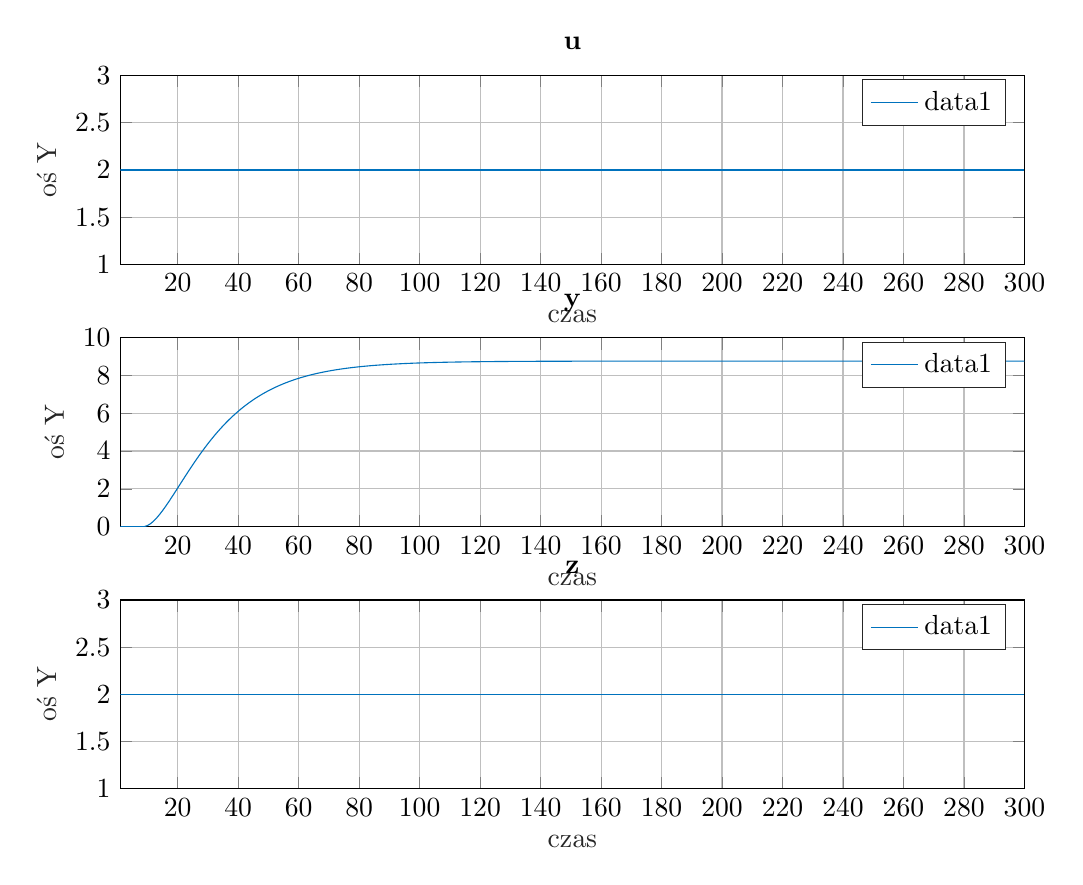
\begin{tikzpicture}

\begin{axis}[%
width=4.521in,
height=0.944in,
at={(0.758in,3.103in)},
scale only axis,
xmin=1,
xmax=300,
xlabel style={font=\color{white!15!black}},
xlabel={czas},
ymin=1,
ymax=3,
ylabel style={font=\color{white!15!black}},
ylabel={oś Y},
axis background/.style={fill=white},
title style={font=\bfseries},
title={u},
xmajorgrids,
ymajorgrids,
legend style={legend cell align=left, align=left, draw=white!15!black}
]
\addplot [color=mycolor1]
  table[row sep=crcr]{%
1	2\\
2	2\\
3	2\\
4	2\\
5	2\\
6	2\\
7	2\\
8	2\\
9	2\\
10	2\\
11	2\\
12	2\\
13	2\\
14	2\\
15	2\\
16	2\\
17	2\\
18	2\\
19	2\\
20	2\\
21	2\\
22	2\\
23	2\\
24	2\\
25	2\\
26	2\\
27	2\\
28	2\\
29	2\\
30	2\\
31	2\\
32	2\\
33	2\\
34	2\\
35	2\\
36	2\\
37	2\\
38	2\\
39	2\\
40	2\\
41	2\\
42	2\\
43	2\\
44	2\\
45	2\\
46	2\\
47	2\\
48	2\\
49	2\\
50	2\\
51	2\\
52	2\\
53	2\\
54	2\\
55	2\\
56	2\\
57	2\\
58	2\\
59	2\\
60	2\\
61	2\\
62	2\\
63	2\\
64	2\\
65	2\\
66	2\\
67	2\\
68	2\\
69	2\\
70	2\\
71	2\\
72	2\\
73	2\\
74	2\\
75	2\\
76	2\\
77	2\\
78	2\\
79	2\\
80	2\\
81	2\\
82	2\\
83	2\\
84	2\\
85	2\\
86	2\\
87	2\\
88	2\\
89	2\\
90	2\\
91	2\\
92	2\\
93	2\\
94	2\\
95	2\\
96	2\\
97	2\\
98	2\\
99	2\\
100	2\\
101	2\\
102	2\\
103	2\\
104	2\\
105	2\\
106	2\\
107	2\\
108	2\\
109	2\\
110	2\\
111	2\\
112	2\\
113	2\\
114	2\\
115	2\\
116	2\\
117	2\\
118	2\\
119	2\\
120	2\\
121	2\\
122	2\\
123	2\\
124	2\\
125	2\\
126	2\\
127	2\\
128	2\\
129	2\\
130	2\\
131	2\\
132	2\\
133	2\\
134	2\\
135	2\\
136	2\\
137	2\\
138	2\\
139	2\\
140	2\\
141	2\\
142	2\\
143	2\\
144	2\\
145	2\\
146	2\\
147	2\\
148	2\\
149	2\\
150	2\\
151	2\\
152	2\\
153	2\\
154	2\\
155	2\\
156	2\\
157	2\\
158	2\\
159	2\\
160	2\\
161	2\\
162	2\\
163	2\\
164	2\\
165	2\\
166	2\\
167	2\\
168	2\\
169	2\\
170	2\\
171	2\\
172	2\\
173	2\\
174	2\\
175	2\\
176	2\\
177	2\\
178	2\\
179	2\\
180	2\\
181	2\\
182	2\\
183	2\\
184	2\\
185	2\\
186	2\\
187	2\\
188	2\\
189	2\\
190	2\\
191	2\\
192	2\\
193	2\\
194	2\\
195	2\\
196	2\\
197	2\\
198	2\\
199	2\\
200	2\\
201	2\\
202	2\\
203	2\\
204	2\\
205	2\\
206	2\\
207	2\\
208	2\\
209	2\\
210	2\\
211	2\\
212	2\\
213	2\\
214	2\\
215	2\\
216	2\\
217	2\\
218	2\\
219	2\\
220	2\\
221	2\\
222	2\\
223	2\\
224	2\\
225	2\\
226	2\\
227	2\\
228	2\\
229	2\\
230	2\\
231	2\\
232	2\\
233	2\\
234	2\\
235	2\\
236	2\\
237	2\\
238	2\\
239	2\\
240	2\\
241	2\\
242	2\\
243	2\\
244	2\\
245	2\\
246	2\\
247	2\\
248	2\\
249	2\\
250	2\\
251	2\\
252	2\\
253	2\\
254	2\\
255	2\\
256	2\\
257	2\\
258	2\\
259	2\\
260	2\\
261	2\\
262	2\\
263	2\\
264	2\\
265	2\\
266	2\\
267	2\\
268	2\\
269	2\\
270	2\\
271	2\\
272	2\\
273	2\\
274	2\\
275	2\\
276	2\\
277	2\\
278	2\\
279	2\\
280	2\\
281	2\\
282	2\\
283	2\\
284	2\\
285	2\\
286	2\\
287	2\\
288	2\\
289	2\\
290	2\\
291	2\\
292	2\\
293	2\\
294	2\\
295	2\\
296	2\\
297	2\\
298	2\\
299	2\\
300	2\\
};
\addlegendentry{data1}

\end{axis}

\begin{axis}[%
width=4.521in,
height=0.944in,
at={(0.758in,1.792in)},
scale only axis,
xmin=1,
xmax=300,
xlabel style={font=\color{white!15!black}},
xlabel={czas},
ymin=0,
ymax=10,
ylabel style={font=\color{white!15!black}},
ylabel={oś Y},
axis background/.style={fill=white},
title style={font=\bfseries},
title={y},
xmajorgrids,
ymajorgrids,
legend style={legend cell align=left, align=left, draw=white!15!black}
]
\addplot [color=mycolor1]
  table[row sep=crcr]{%
1	0\\
2	0\\
3	0\\
4	0\\
5	0\\
6	0\\
7	0\\
8	0\\
9	0\\
10	0.05338\\
11	0.15126\\
12	0.28592\\
13	0.45065\\
14	0.63962\\
15	0.8478\\
16	1.0708\\
17	1.305\\
18	1.5471\\
19	1.7944\\
20	2.0445\\
21	2.2954\\
22	2.5456\\
23	2.7935\\
24	3.0381\\
25	3.2784\\
26	3.5136\\
27	3.7431\\
28	3.9664\\
29	4.1832\\
30	4.3931\\
31	4.5961\\
32	4.7919\\
33	4.9805\\
34	5.162\\
35	5.3363\\
36	5.5036\\
37	5.664\\
38	5.8175\\
39	5.9644\\
40	6.1048\\
41	6.239\\
42	6.367\\
43	6.4891\\
44	6.6055\\
45	6.7164\\
46	6.822\\
47	6.9226\\
48	7.0182\\
49	7.1092\\
50	7.1957\\
51	7.2778\\
52	7.3559\\
53	7.4301\\
54	7.5005\\
55	7.5673\\
56	7.6307\\
57	7.6909\\
58	7.7479\\
59	7.802\\
60	7.8534\\
61	7.902\\
62	7.9481\\
63	7.9918\\
64	8.0332\\
65	8.0724\\
66	8.1096\\
67	8.1448\\
68	8.1782\\
69	8.2097\\
70	8.2396\\
71	8.2679\\
72	8.2947\\
73	8.3201\\
74	8.3441\\
75	8.3669\\
76	8.3884\\
77	8.4088\\
78	8.428\\
79	8.4463\\
80	8.4635\\
81	8.4799\\
82	8.4953\\
83	8.5099\\
84	8.5238\\
85	8.5368\\
86	8.5492\\
87	8.5609\\
88	8.572\\
89	8.5825\\
90	8.5924\\
91	8.6018\\
92	8.6107\\
93	8.6191\\
94	8.627\\
95	8.6345\\
96	8.6416\\
97	8.6483\\
98	8.6547\\
99	8.6607\\
100	8.6664\\
101	8.6717\\
102	8.6768\\
103	8.6816\\
104	8.6862\\
105	8.6905\\
106	8.6945\\
107	8.6984\\
108	8.702\\
109	8.7054\\
110	8.7087\\
111	8.7118\\
112	8.7147\\
113	8.7174\\
114	8.72\\
115	8.7225\\
116	8.7248\\
117	8.727\\
118	8.7291\\
119	8.731\\
120	8.7329\\
121	8.7347\\
122	8.7363\\
123	8.7379\\
124	8.7394\\
125	8.7408\\
126	8.7421\\
127	8.7434\\
128	8.7445\\
129	8.7457\\
130	8.7467\\
131	8.7477\\
132	8.7487\\
133	8.7496\\
134	8.7504\\
135	8.7512\\
136	8.752\\
137	8.7527\\
138	8.7534\\
139	8.754\\
140	8.7546\\
141	8.7552\\
142	8.7558\\
143	8.7563\\
144	8.7568\\
145	8.7572\\
146	8.7577\\
147	8.7581\\
148	8.7585\\
149	8.7588\\
150	8.7592\\
151	8.7595\\
152	8.7598\\
153	8.7601\\
154	8.7604\\
155	8.7606\\
156	8.7609\\
157	8.7611\\
158	8.7613\\
159	8.7615\\
160	8.7617\\
161	8.7619\\
162	8.7621\\
163	8.7623\\
164	8.7624\\
165	8.7626\\
166	8.7627\\
167	8.7629\\
168	8.763\\
169	8.7631\\
170	8.7632\\
171	8.7633\\
172	8.7634\\
173	8.7635\\
174	8.7636\\
175	8.7637\\
176	8.7638\\
177	8.7639\\
178	8.7639\\
179	8.764\\
180	8.7641\\
181	8.7641\\
182	8.7642\\
183	8.7642\\
184	8.7643\\
185	8.7643\\
186	8.7644\\
187	8.7644\\
188	8.7645\\
189	8.7645\\
190	8.7645\\
191	8.7646\\
192	8.7646\\
193	8.7646\\
194	8.7647\\
195	8.7647\\
196	8.7647\\
197	8.7648\\
198	8.7648\\
199	8.7648\\
200	8.7648\\
201	8.7648\\
202	8.7649\\
203	8.7649\\
204	8.7649\\
205	8.7649\\
206	8.7649\\
207	8.7649\\
208	8.765\\
209	8.765\\
210	8.765\\
211	8.765\\
212	8.765\\
213	8.765\\
214	8.765\\
215	8.765\\
216	8.765\\
217	8.765\\
218	8.7651\\
219	8.7651\\
220	8.7651\\
221	8.7651\\
222	8.7651\\
223	8.7651\\
224	8.7651\\
225	8.7651\\
226	8.7651\\
227	8.7651\\
228	8.7651\\
229	8.7651\\
230	8.7651\\
231	8.7651\\
232	8.7651\\
233	8.7651\\
234	8.7651\\
235	8.7651\\
236	8.7651\\
237	8.7651\\
238	8.7651\\
239	8.7651\\
240	8.7651\\
241	8.7652\\
242	8.7652\\
243	8.7652\\
244	8.7652\\
245	8.7652\\
246	8.7652\\
247	8.7652\\
248	8.7652\\
249	8.7652\\
250	8.7652\\
251	8.7652\\
252	8.7652\\
253	8.7652\\
254	8.7652\\
255	8.7652\\
256	8.7652\\
257	8.7652\\
258	8.7652\\
259	8.7652\\
260	8.7652\\
261	8.7652\\
262	8.7652\\
263	8.7652\\
264	8.7652\\
265	8.7652\\
266	8.7652\\
267	8.7652\\
268	8.7652\\
269	8.7652\\
270	8.7652\\
271	8.7652\\
272	8.7652\\
273	8.7652\\
274	8.7652\\
275	8.7652\\
276	8.7652\\
277	8.7652\\
278	8.7652\\
279	8.7652\\
280	8.7652\\
281	8.7652\\
282	8.7652\\
283	8.7652\\
284	8.7652\\
285	8.7652\\
286	8.7652\\
287	8.7652\\
288	8.7652\\
289	8.7652\\
290	8.7652\\
291	8.7652\\
292	8.7652\\
293	8.7652\\
294	8.7652\\
295	8.7652\\
296	8.7652\\
297	8.7652\\
298	8.7652\\
299	8.7652\\
300	8.7652\\
};
\addlegendentry{data1}

\end{axis}

\begin{axis}[%
width=4.521in,
height=0.944in,
at={(0.758in,0.481in)},
scale only axis,
xmin=1,
xmax=300,
xlabel style={font=\color{white!15!black}},
xlabel={czas},
ymin=1,
ymax=3,
ylabel style={font=\color{white!15!black}},
ylabel={oś Y},
axis background/.style={fill=white},
title style={font=\bfseries},
title={z},
xmajorgrids,
ymajorgrids,
legend style={legend cell align=left, align=left, draw=white!15!black}
]
\addplot [color=mycolor1]
  table[row sep=crcr]{%
1	2\\
2	2\\
3	2\\
4	2\\
5	2\\
6	2\\
7	2\\
8	2\\
9	2\\
10	2\\
11	2\\
12	2\\
13	2\\
14	2\\
15	2\\
16	2\\
17	2\\
18	2\\
19	2\\
20	2\\
21	2\\
22	2\\
23	2\\
24	2\\
25	2\\
26	2\\
27	2\\
28	2\\
29	2\\
30	2\\
31	2\\
32	2\\
33	2\\
34	2\\
35	2\\
36	2\\
37	2\\
38	2\\
39	2\\
40	2\\
41	2\\
42	2\\
43	2\\
44	2\\
45	2\\
46	2\\
47	2\\
48	2\\
49	2\\
50	2\\
51	2\\
52	2\\
53	2\\
54	2\\
55	2\\
56	2\\
57	2\\
58	2\\
59	2\\
60	2\\
61	2\\
62	2\\
63	2\\
64	2\\
65	2\\
66	2\\
67	2\\
68	2\\
69	2\\
70	2\\
71	2\\
72	2\\
73	2\\
74	2\\
75	2\\
76	2\\
77	2\\
78	2\\
79	2\\
80	2\\
81	2\\
82	2\\
83	2\\
84	2\\
85	2\\
86	2\\
87	2\\
88	2\\
89	2\\
90	2\\
91	2\\
92	2\\
93	2\\
94	2\\
95	2\\
96	2\\
97	2\\
98	2\\
99	2\\
100	2\\
101	2\\
102	2\\
103	2\\
104	2\\
105	2\\
106	2\\
107	2\\
108	2\\
109	2\\
110	2\\
111	2\\
112	2\\
113	2\\
114	2\\
115	2\\
116	2\\
117	2\\
118	2\\
119	2\\
120	2\\
121	2\\
122	2\\
123	2\\
124	2\\
125	2\\
126	2\\
127	2\\
128	2\\
129	2\\
130	2\\
131	2\\
132	2\\
133	2\\
134	2\\
135	2\\
136	2\\
137	2\\
138	2\\
139	2\\
140	2\\
141	2\\
142	2\\
143	2\\
144	2\\
145	2\\
146	2\\
147	2\\
148	2\\
149	2\\
150	2\\
151	2\\
152	2\\
153	2\\
154	2\\
155	2\\
156	2\\
157	2\\
158	2\\
159	2\\
160	2\\
161	2\\
162	2\\
163	2\\
164	2\\
165	2\\
166	2\\
167	2\\
168	2\\
169	2\\
170	2\\
171	2\\
172	2\\
173	2\\
174	2\\
175	2\\
176	2\\
177	2\\
178	2\\
179	2\\
180	2\\
181	2\\
182	2\\
183	2\\
184	2\\
185	2\\
186	2\\
187	2\\
188	2\\
189	2\\
190	2\\
191	2\\
192	2\\
193	2\\
194	2\\
195	2\\
196	2\\
197	2\\
198	2\\
199	2\\
200	2\\
201	2\\
202	2\\
203	2\\
204	2\\
205	2\\
206	2\\
207	2\\
208	2\\
209	2\\
210	2\\
211	2\\
212	2\\
213	2\\
214	2\\
215	2\\
216	2\\
217	2\\
218	2\\
219	2\\
220	2\\
221	2\\
222	2\\
223	2\\
224	2\\
225	2\\
226	2\\
227	2\\
228	2\\
229	2\\
230	2\\
231	2\\
232	2\\
233	2\\
234	2\\
235	2\\
236	2\\
237	2\\
238	2\\
239	2\\
240	2\\
241	2\\
242	2\\
243	2\\
244	2\\
245	2\\
246	2\\
247	2\\
248	2\\
249	2\\
250	2\\
251	2\\
252	2\\
253	2\\
254	2\\
255	2\\
256	2\\
257	2\\
258	2\\
259	2\\
260	2\\
261	2\\
262	2\\
263	2\\
264	2\\
265	2\\
266	2\\
267	2\\
268	2\\
269	2\\
270	2\\
271	2\\
272	2\\
273	2\\
274	2\\
275	2\\
276	2\\
277	2\\
278	2\\
279	2\\
280	2\\
281	2\\
282	2\\
283	2\\
284	2\\
285	2\\
286	2\\
287	2\\
288	2\\
289	2\\
290	2\\
291	2\\
292	2\\
293	2\\
294	2\\
295	2\\
296	2\\
297	2\\
298	2\\
299	2\\
300	2\\
};
\addlegendentry{data1}

\end{axis}
\end{tikzpicture}%

koniec wykresu

dwa subploty

% This file was created by matlab2tikz.
%
\definecolor{mycolor1}{rgb}{0.00000,0.44700,0.74100}%
%
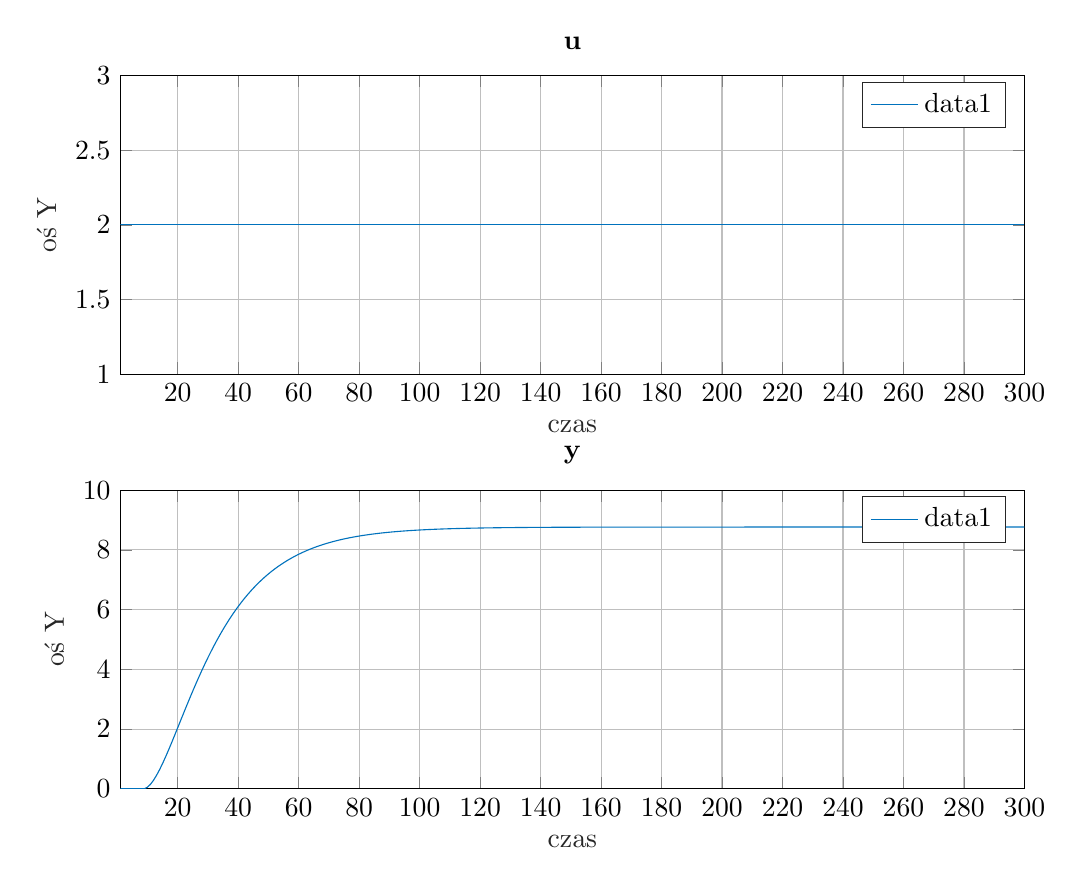
\begin{tikzpicture}

\begin{axis}[%
width=4.521in,
height=1.493in,
at={(0.758in,2.554in)},
scale only axis,
xmin=1,
xmax=300,
xlabel style={font=\color{white!15!black}},
xlabel={czas},
ymin=1,
ymax=3,
ylabel style={font=\color{white!15!black}},
ylabel={oś Y},
axis background/.style={fill=white},
title style={font=\bfseries},
title={u},
xmajorgrids,
ymajorgrids,
legend style={legend cell align=left, align=left, draw=white!15!black}
]
\addplot [color=mycolor1]
  table[row sep=crcr]{%
1	2\\
2	2\\
3	2\\
4	2\\
5	2\\
6	2\\
7	2\\
8	2\\
9	2\\
10	2\\
11	2\\
12	2\\
13	2\\
14	2\\
15	2\\
16	2\\
17	2\\
18	2\\
19	2\\
20	2\\
21	2\\
22	2\\
23	2\\
24	2\\
25	2\\
26	2\\
27	2\\
28	2\\
29	2\\
30	2\\
31	2\\
32	2\\
33	2\\
34	2\\
35	2\\
36	2\\
37	2\\
38	2\\
39	2\\
40	2\\
41	2\\
42	2\\
43	2\\
44	2\\
45	2\\
46	2\\
47	2\\
48	2\\
49	2\\
50	2\\
51	2\\
52	2\\
53	2\\
54	2\\
55	2\\
56	2\\
57	2\\
58	2\\
59	2\\
60	2\\
61	2\\
62	2\\
63	2\\
64	2\\
65	2\\
66	2\\
67	2\\
68	2\\
69	2\\
70	2\\
71	2\\
72	2\\
73	2\\
74	2\\
75	2\\
76	2\\
77	2\\
78	2\\
79	2\\
80	2\\
81	2\\
82	2\\
83	2\\
84	2\\
85	2\\
86	2\\
87	2\\
88	2\\
89	2\\
90	2\\
91	2\\
92	2\\
93	2\\
94	2\\
95	2\\
96	2\\
97	2\\
98	2\\
99	2\\
100	2\\
101	2\\
102	2\\
103	2\\
104	2\\
105	2\\
106	2\\
107	2\\
108	2\\
109	2\\
110	2\\
111	2\\
112	2\\
113	2\\
114	2\\
115	2\\
116	2\\
117	2\\
118	2\\
119	2\\
120	2\\
121	2\\
122	2\\
123	2\\
124	2\\
125	2\\
126	2\\
127	2\\
128	2\\
129	2\\
130	2\\
131	2\\
132	2\\
133	2\\
134	2\\
135	2\\
136	2\\
137	2\\
138	2\\
139	2\\
140	2\\
141	2\\
142	2\\
143	2\\
144	2\\
145	2\\
146	2\\
147	2\\
148	2\\
149	2\\
150	2\\
151	2\\
152	2\\
153	2\\
154	2\\
155	2\\
156	2\\
157	2\\
158	2\\
159	2\\
160	2\\
161	2\\
162	2\\
163	2\\
164	2\\
165	2\\
166	2\\
167	2\\
168	2\\
169	2\\
170	2\\
171	2\\
172	2\\
173	2\\
174	2\\
175	2\\
176	2\\
177	2\\
178	2\\
179	2\\
180	2\\
181	2\\
182	2\\
183	2\\
184	2\\
185	2\\
186	2\\
187	2\\
188	2\\
189	2\\
190	2\\
191	2\\
192	2\\
193	2\\
194	2\\
195	2\\
196	2\\
197	2\\
198	2\\
199	2\\
200	2\\
201	2\\
202	2\\
203	2\\
204	2\\
205	2\\
206	2\\
207	2\\
208	2\\
209	2\\
210	2\\
211	2\\
212	2\\
213	2\\
214	2\\
215	2\\
216	2\\
217	2\\
218	2\\
219	2\\
220	2\\
221	2\\
222	2\\
223	2\\
224	2\\
225	2\\
226	2\\
227	2\\
228	2\\
229	2\\
230	2\\
231	2\\
232	2\\
233	2\\
234	2\\
235	2\\
236	2\\
237	2\\
238	2\\
239	2\\
240	2\\
241	2\\
242	2\\
243	2\\
244	2\\
245	2\\
246	2\\
247	2\\
248	2\\
249	2\\
250	2\\
251	2\\
252	2\\
253	2\\
254	2\\
255	2\\
256	2\\
257	2\\
258	2\\
259	2\\
260	2\\
261	2\\
262	2\\
263	2\\
264	2\\
265	2\\
266	2\\
267	2\\
268	2\\
269	2\\
270	2\\
271	2\\
272	2\\
273	2\\
274	2\\
275	2\\
276	2\\
277	2\\
278	2\\
279	2\\
280	2\\
281	2\\
282	2\\
283	2\\
284	2\\
285	2\\
286	2\\
287	2\\
288	2\\
289	2\\
290	2\\
291	2\\
292	2\\
293	2\\
294	2\\
295	2\\
296	2\\
297	2\\
298	2\\
299	2\\
300	2\\
};
\addlegendentry{data1}

\end{axis}

\begin{axis}[%
width=4.521in,
height=1.493in,
at={(0.758in,0.481in)},
scale only axis,
xmin=1,
xmax=300,
xlabel style={font=\color{white!15!black}},
xlabel={czas},
ymin=0,
ymax=10,
ylabel style={font=\color{white!15!black}},
ylabel={oś Y},
axis background/.style={fill=white},
title style={font=\bfseries},
title={y},
xmajorgrids,
ymajorgrids,
legend style={legend cell align=left, align=left, draw=white!15!black}
]
\addplot [color=mycolor1]
  table[row sep=crcr]{%
1	0\\
2	0\\
3	0\\
4	0\\
5	0\\
6	0\\
7	0\\
8	0\\
9	0\\
10	0.05338\\
11	0.15126\\
12	0.28592\\
13	0.45065\\
14	0.63962\\
15	0.8478\\
16	1.0708\\
17	1.305\\
18	1.5471\\
19	1.7944\\
20	2.0445\\
21	2.2954\\
22	2.5456\\
23	2.7935\\
24	3.0381\\
25	3.2784\\
26	3.5136\\
27	3.7431\\
28	3.9664\\
29	4.1832\\
30	4.3931\\
31	4.5961\\
32	4.7919\\
33	4.9805\\
34	5.162\\
35	5.3363\\
36	5.5036\\
37	5.664\\
38	5.8175\\
39	5.9644\\
40	6.1048\\
41	6.239\\
42	6.367\\
43	6.4891\\
44	6.6055\\
45	6.7164\\
46	6.822\\
47	6.9226\\
48	7.0182\\
49	7.1092\\
50	7.1957\\
51	7.2778\\
52	7.3559\\
53	7.4301\\
54	7.5005\\
55	7.5673\\
56	7.6307\\
57	7.6909\\
58	7.7479\\
59	7.802\\
60	7.8534\\
61	7.902\\
62	7.9481\\
63	7.9918\\
64	8.0332\\
65	8.0724\\
66	8.1096\\
67	8.1448\\
68	8.1782\\
69	8.2097\\
70	8.2396\\
71	8.2679\\
72	8.2947\\
73	8.3201\\
74	8.3441\\
75	8.3669\\
76	8.3884\\
77	8.4088\\
78	8.428\\
79	8.4463\\
80	8.4635\\
81	8.4799\\
82	8.4953\\
83	8.5099\\
84	8.5238\\
85	8.5368\\
86	8.5492\\
87	8.5609\\
88	8.572\\
89	8.5825\\
90	8.5924\\
91	8.6018\\
92	8.6107\\
93	8.6191\\
94	8.627\\
95	8.6345\\
96	8.6416\\
97	8.6483\\
98	8.6547\\
99	8.6607\\
100	8.6664\\
101	8.6717\\
102	8.6768\\
103	8.6816\\
104	8.6862\\
105	8.6905\\
106	8.6945\\
107	8.6984\\
108	8.702\\
109	8.7054\\
110	8.7087\\
111	8.7118\\
112	8.7147\\
113	8.7174\\
114	8.72\\
115	8.7225\\
116	8.7248\\
117	8.727\\
118	8.7291\\
119	8.731\\
120	8.7329\\
121	8.7347\\
122	8.7363\\
123	8.7379\\
124	8.7394\\
125	8.7408\\
126	8.7421\\
127	8.7434\\
128	8.7445\\
129	8.7457\\
130	8.7467\\
131	8.7477\\
132	8.7487\\
133	8.7496\\
134	8.7504\\
135	8.7512\\
136	8.752\\
137	8.7527\\
138	8.7534\\
139	8.754\\
140	8.7546\\
141	8.7552\\
142	8.7558\\
143	8.7563\\
144	8.7568\\
145	8.7572\\
146	8.7577\\
147	8.7581\\
148	8.7585\\
149	8.7588\\
150	8.7592\\
151	8.7595\\
152	8.7598\\
153	8.7601\\
154	8.7604\\
155	8.7606\\
156	8.7609\\
157	8.7611\\
158	8.7613\\
159	8.7615\\
160	8.7617\\
161	8.7619\\
162	8.7621\\
163	8.7623\\
164	8.7624\\
165	8.7626\\
166	8.7627\\
167	8.7629\\
168	8.763\\
169	8.7631\\
170	8.7632\\
171	8.7633\\
172	8.7634\\
173	8.7635\\
174	8.7636\\
175	8.7637\\
176	8.7638\\
177	8.7639\\
178	8.7639\\
179	8.764\\
180	8.7641\\
181	8.7641\\
182	8.7642\\
183	8.7642\\
184	8.7643\\
185	8.7643\\
186	8.7644\\
187	8.7644\\
188	8.7645\\
189	8.7645\\
190	8.7645\\
191	8.7646\\
192	8.7646\\
193	8.7646\\
194	8.7647\\
195	8.7647\\
196	8.7647\\
197	8.7648\\
198	8.7648\\
199	8.7648\\
200	8.7648\\
201	8.7648\\
202	8.7649\\
203	8.7649\\
204	8.7649\\
205	8.7649\\
206	8.7649\\
207	8.7649\\
208	8.765\\
209	8.765\\
210	8.765\\
211	8.765\\
212	8.765\\
213	8.765\\
214	8.765\\
215	8.765\\
216	8.765\\
217	8.765\\
218	8.7651\\
219	8.7651\\
220	8.7651\\
221	8.7651\\
222	8.7651\\
223	8.7651\\
224	8.7651\\
225	8.7651\\
226	8.7651\\
227	8.7651\\
228	8.7651\\
229	8.7651\\
230	8.7651\\
231	8.7651\\
232	8.7651\\
233	8.7651\\
234	8.7651\\
235	8.7651\\
236	8.7651\\
237	8.7651\\
238	8.7651\\
239	8.7651\\
240	8.7651\\
241	8.7652\\
242	8.7652\\
243	8.7652\\
244	8.7652\\
245	8.7652\\
246	8.7652\\
247	8.7652\\
248	8.7652\\
249	8.7652\\
250	8.7652\\
251	8.7652\\
252	8.7652\\
253	8.7652\\
254	8.7652\\
255	8.7652\\
256	8.7652\\
257	8.7652\\
258	8.7652\\
259	8.7652\\
260	8.7652\\
261	8.7652\\
262	8.7652\\
263	8.7652\\
264	8.7652\\
265	8.7652\\
266	8.7652\\
267	8.7652\\
268	8.7652\\
269	8.7652\\
270	8.7652\\
271	8.7652\\
272	8.7652\\
273	8.7652\\
274	8.7652\\
275	8.7652\\
276	8.7652\\
277	8.7652\\
278	8.7652\\
279	8.7652\\
280	8.7652\\
281	8.7652\\
282	8.7652\\
283	8.7652\\
284	8.7652\\
285	8.7652\\
286	8.7652\\
287	8.7652\\
288	8.7652\\
289	8.7652\\
290	8.7652\\
291	8.7652\\
292	8.7652\\
293	8.7652\\
294	8.7652\\
295	8.7652\\
296	8.7652\\
297	8.7652\\
298	8.7652\\
299	8.7652\\
300	8.7652\\
};
\addlegendentry{data1}

\end{axis}
\end{tikzpicture}%

koniec wykresu

jeden plot

% This file was created by matlab2tikz.
%
\definecolor{mycolor1}{rgb}{0.00000,0.44700,0.74100}%
%
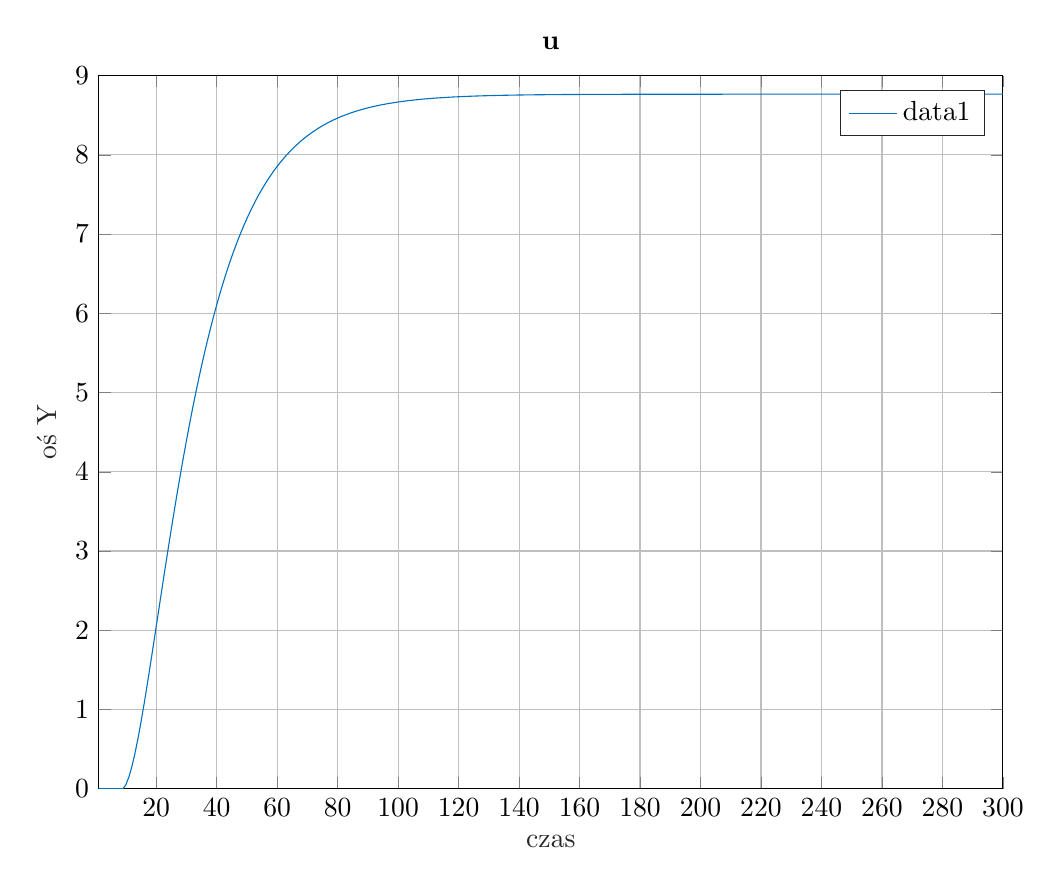
\begin{tikzpicture}

\begin{axis}[%
width=4.521in,
height=3.566in,
at={(0.758in,0.481in)},
scale only axis,
xmin=1,
xmax=300,
xlabel style={font=\color{white!15!black}},
xlabel={czas},
ymin=0,
ymax=9,
ylabel style={font=\color{white!15!black}},
ylabel={oś Y},
axis background/.style={fill=white},
title style={font=\bfseries},
title={u},
xmajorgrids,
ymajorgrids,
legend style={legend cell align=left, align=left, draw=white!15!black}
]
\addplot [color=mycolor1]
  table[row sep=crcr]{%
1	0\\
2	0\\
3	0\\
4	0\\
5	0\\
6	0\\
7	0\\
8	0\\
9	0\\
10	0.05338\\
11	0.15126\\
12	0.28592\\
13	0.45065\\
14	0.63962\\
15	0.8478\\
16	1.0708\\
17	1.305\\
18	1.5471\\
19	1.7944\\
20	2.0445\\
21	2.2954\\
22	2.5456\\
23	2.7935\\
24	3.0381\\
25	3.2784\\
26	3.5136\\
27	3.7431\\
28	3.9664\\
29	4.1832\\
30	4.3931\\
31	4.5961\\
32	4.7919\\
33	4.9805\\
34	5.162\\
35	5.3363\\
36	5.5036\\
37	5.664\\
38	5.8175\\
39	5.9644\\
40	6.1048\\
41	6.239\\
42	6.367\\
43	6.4891\\
44	6.6055\\
45	6.7164\\
46	6.822\\
47	6.9226\\
48	7.0182\\
49	7.1092\\
50	7.1957\\
51	7.2778\\
52	7.3559\\
53	7.4301\\
54	7.5005\\
55	7.5673\\
56	7.6307\\
57	7.6909\\
58	7.7479\\
59	7.802\\
60	7.8534\\
61	7.902\\
62	7.9481\\
63	7.9918\\
64	8.0332\\
65	8.0724\\
66	8.1096\\
67	8.1448\\
68	8.1782\\
69	8.2097\\
70	8.2396\\
71	8.2679\\
72	8.2947\\
73	8.3201\\
74	8.3441\\
75	8.3669\\
76	8.3884\\
77	8.4088\\
78	8.428\\
79	8.4463\\
80	8.4635\\
81	8.4799\\
82	8.4953\\
83	8.5099\\
84	8.5238\\
85	8.5368\\
86	8.5492\\
87	8.5609\\
88	8.572\\
89	8.5825\\
90	8.5924\\
91	8.6018\\
92	8.6107\\
93	8.6191\\
94	8.627\\
95	8.6345\\
96	8.6416\\
97	8.6483\\
98	8.6547\\
99	8.6607\\
100	8.6664\\
101	8.6717\\
102	8.6768\\
103	8.6816\\
104	8.6862\\
105	8.6905\\
106	8.6945\\
107	8.6984\\
108	8.702\\
109	8.7054\\
110	8.7087\\
111	8.7118\\
112	8.7147\\
113	8.7174\\
114	8.72\\
115	8.7225\\
116	8.7248\\
117	8.727\\
118	8.7291\\
119	8.731\\
120	8.7329\\
121	8.7347\\
122	8.7363\\
123	8.7379\\
124	8.7394\\
125	8.7408\\
126	8.7421\\
127	8.7434\\
128	8.7445\\
129	8.7457\\
130	8.7467\\
131	8.7477\\
132	8.7487\\
133	8.7496\\
134	8.7504\\
135	8.7512\\
136	8.752\\
137	8.7527\\
138	8.7534\\
139	8.754\\
140	8.7546\\
141	8.7552\\
142	8.7558\\
143	8.7563\\
144	8.7568\\
145	8.7572\\
146	8.7577\\
147	8.7581\\
148	8.7585\\
149	8.7588\\
150	8.7592\\
151	8.7595\\
152	8.7598\\
153	8.7601\\
154	8.7604\\
155	8.7606\\
156	8.7609\\
157	8.7611\\
158	8.7613\\
159	8.7615\\
160	8.7617\\
161	8.7619\\
162	8.7621\\
163	8.7623\\
164	8.7624\\
165	8.7626\\
166	8.7627\\
167	8.7629\\
168	8.763\\
169	8.7631\\
170	8.7632\\
171	8.7633\\
172	8.7634\\
173	8.7635\\
174	8.7636\\
175	8.7637\\
176	8.7638\\
177	8.7639\\
178	8.7639\\
179	8.764\\
180	8.7641\\
181	8.7641\\
182	8.7642\\
183	8.7642\\
184	8.7643\\
185	8.7643\\
186	8.7644\\
187	8.7644\\
188	8.7645\\
189	8.7645\\
190	8.7645\\
191	8.7646\\
192	8.7646\\
193	8.7646\\
194	8.7647\\
195	8.7647\\
196	8.7647\\
197	8.7648\\
198	8.7648\\
199	8.7648\\
200	8.7648\\
201	8.7648\\
202	8.7649\\
203	8.7649\\
204	8.7649\\
205	8.7649\\
206	8.7649\\
207	8.7649\\
208	8.765\\
209	8.765\\
210	8.765\\
211	8.765\\
212	8.765\\
213	8.765\\
214	8.765\\
215	8.765\\
216	8.765\\
217	8.765\\
218	8.7651\\
219	8.7651\\
220	8.7651\\
221	8.7651\\
222	8.7651\\
223	8.7651\\
224	8.7651\\
225	8.7651\\
226	8.7651\\
227	8.7651\\
228	8.7651\\
229	8.7651\\
230	8.7651\\
231	8.7651\\
232	8.7651\\
233	8.7651\\
234	8.7651\\
235	8.7651\\
236	8.7651\\
237	8.7651\\
238	8.7651\\
239	8.7651\\
240	8.7651\\
241	8.7652\\
242	8.7652\\
243	8.7652\\
244	8.7652\\
245	8.7652\\
246	8.7652\\
247	8.7652\\
248	8.7652\\
249	8.7652\\
250	8.7652\\
251	8.7652\\
252	8.7652\\
253	8.7652\\
254	8.7652\\
255	8.7652\\
256	8.7652\\
257	8.7652\\
258	8.7652\\
259	8.7652\\
260	8.7652\\
261	8.7652\\
262	8.7652\\
263	8.7652\\
264	8.7652\\
265	8.7652\\
266	8.7652\\
267	8.7652\\
268	8.7652\\
269	8.7652\\
270	8.7652\\
271	8.7652\\
272	8.7652\\
273	8.7652\\
274	8.7652\\
275	8.7652\\
276	8.7652\\
277	8.7652\\
278	8.7652\\
279	8.7652\\
280	8.7652\\
281	8.7652\\
282	8.7652\\
283	8.7652\\
284	8.7652\\
285	8.7652\\
286	8.7652\\
287	8.7652\\
288	8.7652\\
289	8.7652\\
290	8.7652\\
291	8.7652\\
292	8.7652\\
293	8.7652\\
294	8.7652\\
295	8.7652\\
296	8.7652\\
297	8.7652\\
298	8.7652\\
299	8.7652\\
300	8.7652\\
};
\addlegendentry{data1}

\end{axis}
\end{tikzpicture}%

koniec wykresu 

\subsection{Odpowiedź wyjścia na skok zakłócenia}
